\chapter{Exploiting Software Diversification for \Wasm}
\label{exploit}



\chapterprecishere{If you find that you're spending all your time on theory, start turning some attention to practical things; it will improve your theories. If you find that you're spending almost all your time on practice, start turning some attention to theoretical things; it will improve your practice.\par\raggedleft--- {\small\textup{Donald Knuth}}}

\vspace{12mm}

\lettrine[lines=3]{I}{n} this chapter, we illustrate the application of Software Diversification for both offensive and defensive purposes.
We discuss two selected use cases that demonstrate practical applications of our contributions.




\msection{Offensive Diversification: Malware evasion}
\label{offensive_app}

The primary malicious use of WebAssembly in browsers is cryptojacking \cite{musch2019new}. 
This is due to the essence of cryptojacking, the faster the mining, the better. 
Let us illustrate how a malicious \Wasm binary is involved into browser cryptojacking.
\autoref{fig:attack_crypto} illustrates a browser attack scenario:
a practical WebAssembly cryptojacking attack consists of three components: a WebAssembly binary, a JavaScript wrapper, and a backend cryptominer pool. 
The WebAssembly binary is responsible for executing the hash calculations, which consume significant computational resources. 
The JavaScript wrapper facilitates the communication between the WebAssembly binary and the cryptominer pool.

\begin{figure}[h]
    \centering
    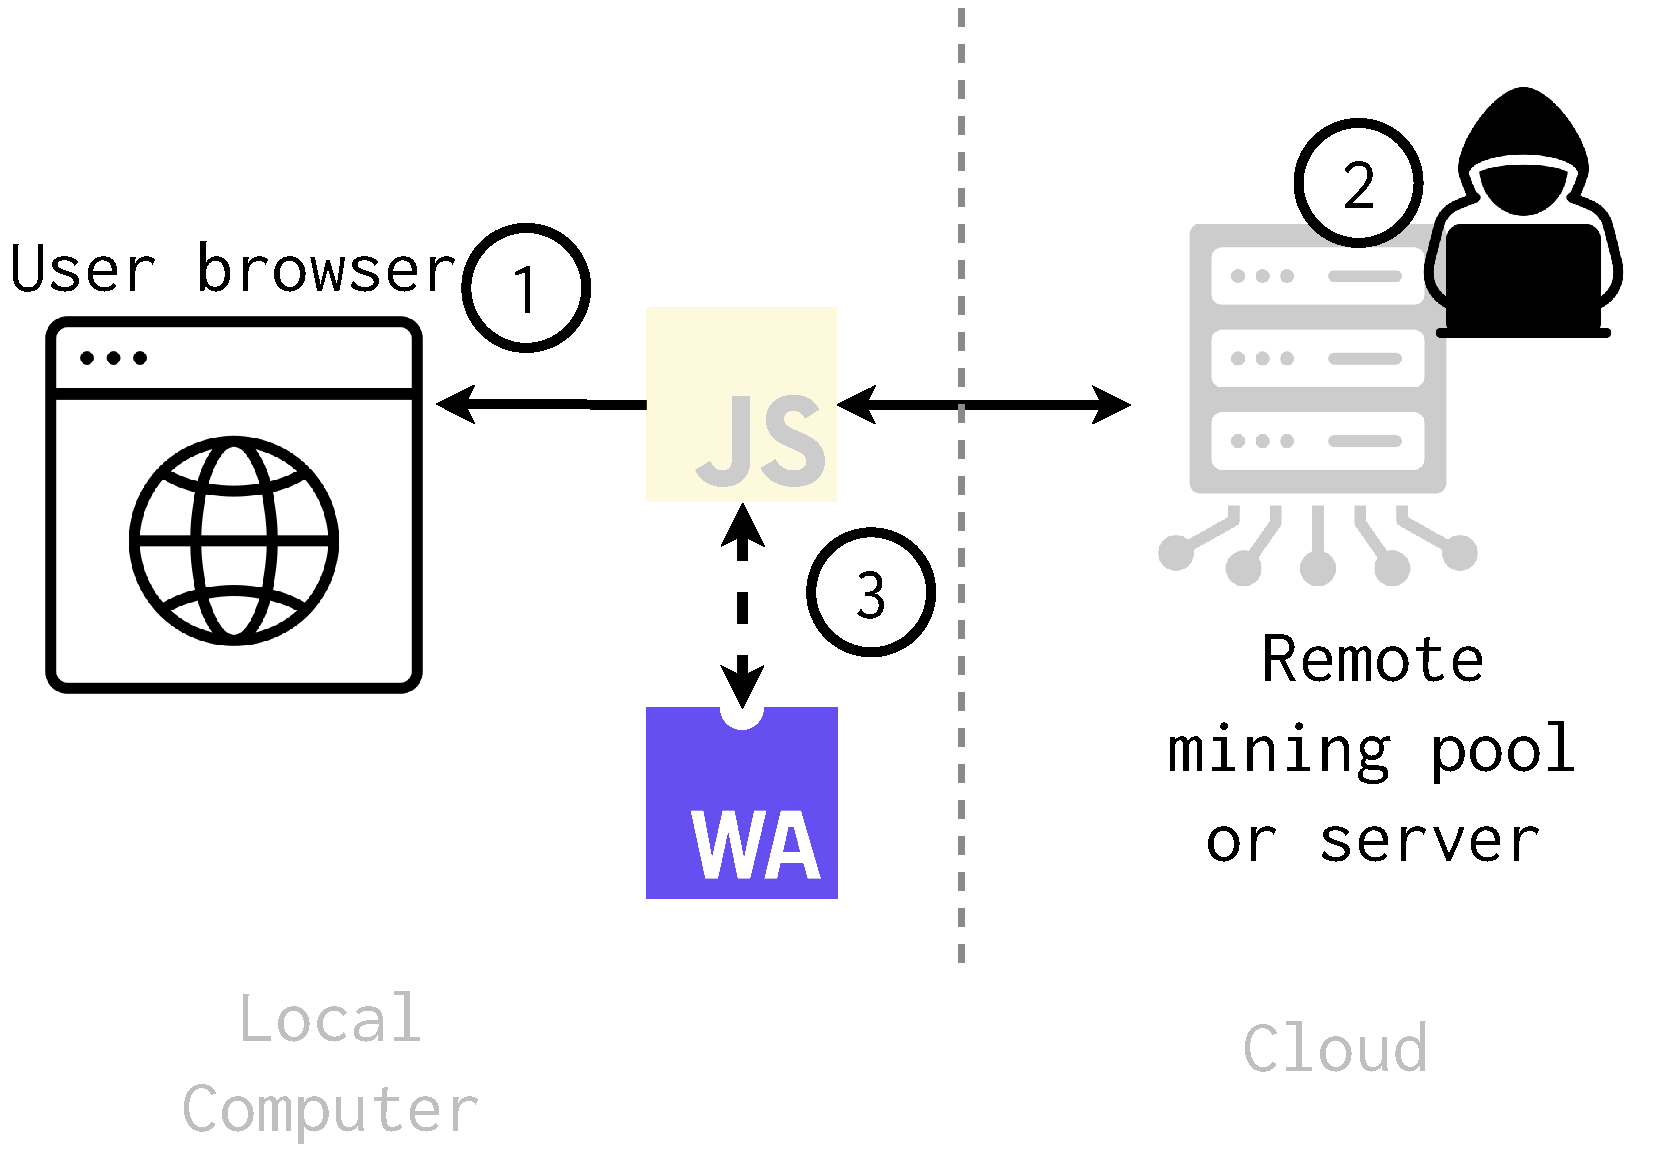
\includegraphics[width=0.6\linewidth]{figures/attack_crypto.pdf}
    \caption{A remote mining pool server, a JavaScript wrapper and the \Wasm binary form the triad of a cryptojacking attack in browser clients.}
    \label{fig:attack_crypto}
\end{figure}

The aforementioned components require the following steps to succeed in cryptomining.
First, the victim visits a web page infected with the cryptojacking code. 
The web page establishes a channel to the cryptominer pool, which then assigns a hashing job to the infected browser. 
The WebAssembly cryptominer calculates thousands of hashes inside the browser. 
Once the malware server receives acceptable hashes, it is rewarded with cryptocurrencies for the mining. 
Then, the server assigns a new job, and the mining process starts over.

Both antivirus software and browsers have implemented measures to detect cryptojacking. For instance, Firefox employs deny lists to detect cryptomining activities \cite{firefoxcrypto}. 
The academic community has also contributed to the body of work on detecting or preventing WebAssembly-based cryptojacking, as outlined in \autoref{background:wasm:analysis}. 
However, malicious actors can employ evasion techniques to circumvent these detection mechanisms. 
Bhansali \etal are among the first who have investigated how WebAssembly cryptojacking could potentially evade detection \cite{10.1145/3507657.3528560}, highlighting the critical importance of this use case. 
The case illustrated in the subsequent sections uses Offensive Software Diversification for evading malware detection in \Wasm. 

\msubsection{Cryptojacking defense evasion}
\label{threat_model}


Considering the previous scenario, several techniques can be directly implemented in browsers to thwart cryptojacking by identifying the malicious \Wasm components. 
Such defense scenario is illustrated in \autoref{fig:threat_model}, where the \Wasm malicious binary is blocked in \step{3}.
The primary aim of our use case is to investigate the effectiveness of code diversification as a means to circumvent cryptojacking defenses. 
Specifically, we assess whether the following evasion workflow can successfully bypass existing security measures:

\begin{figure}
    \centering
    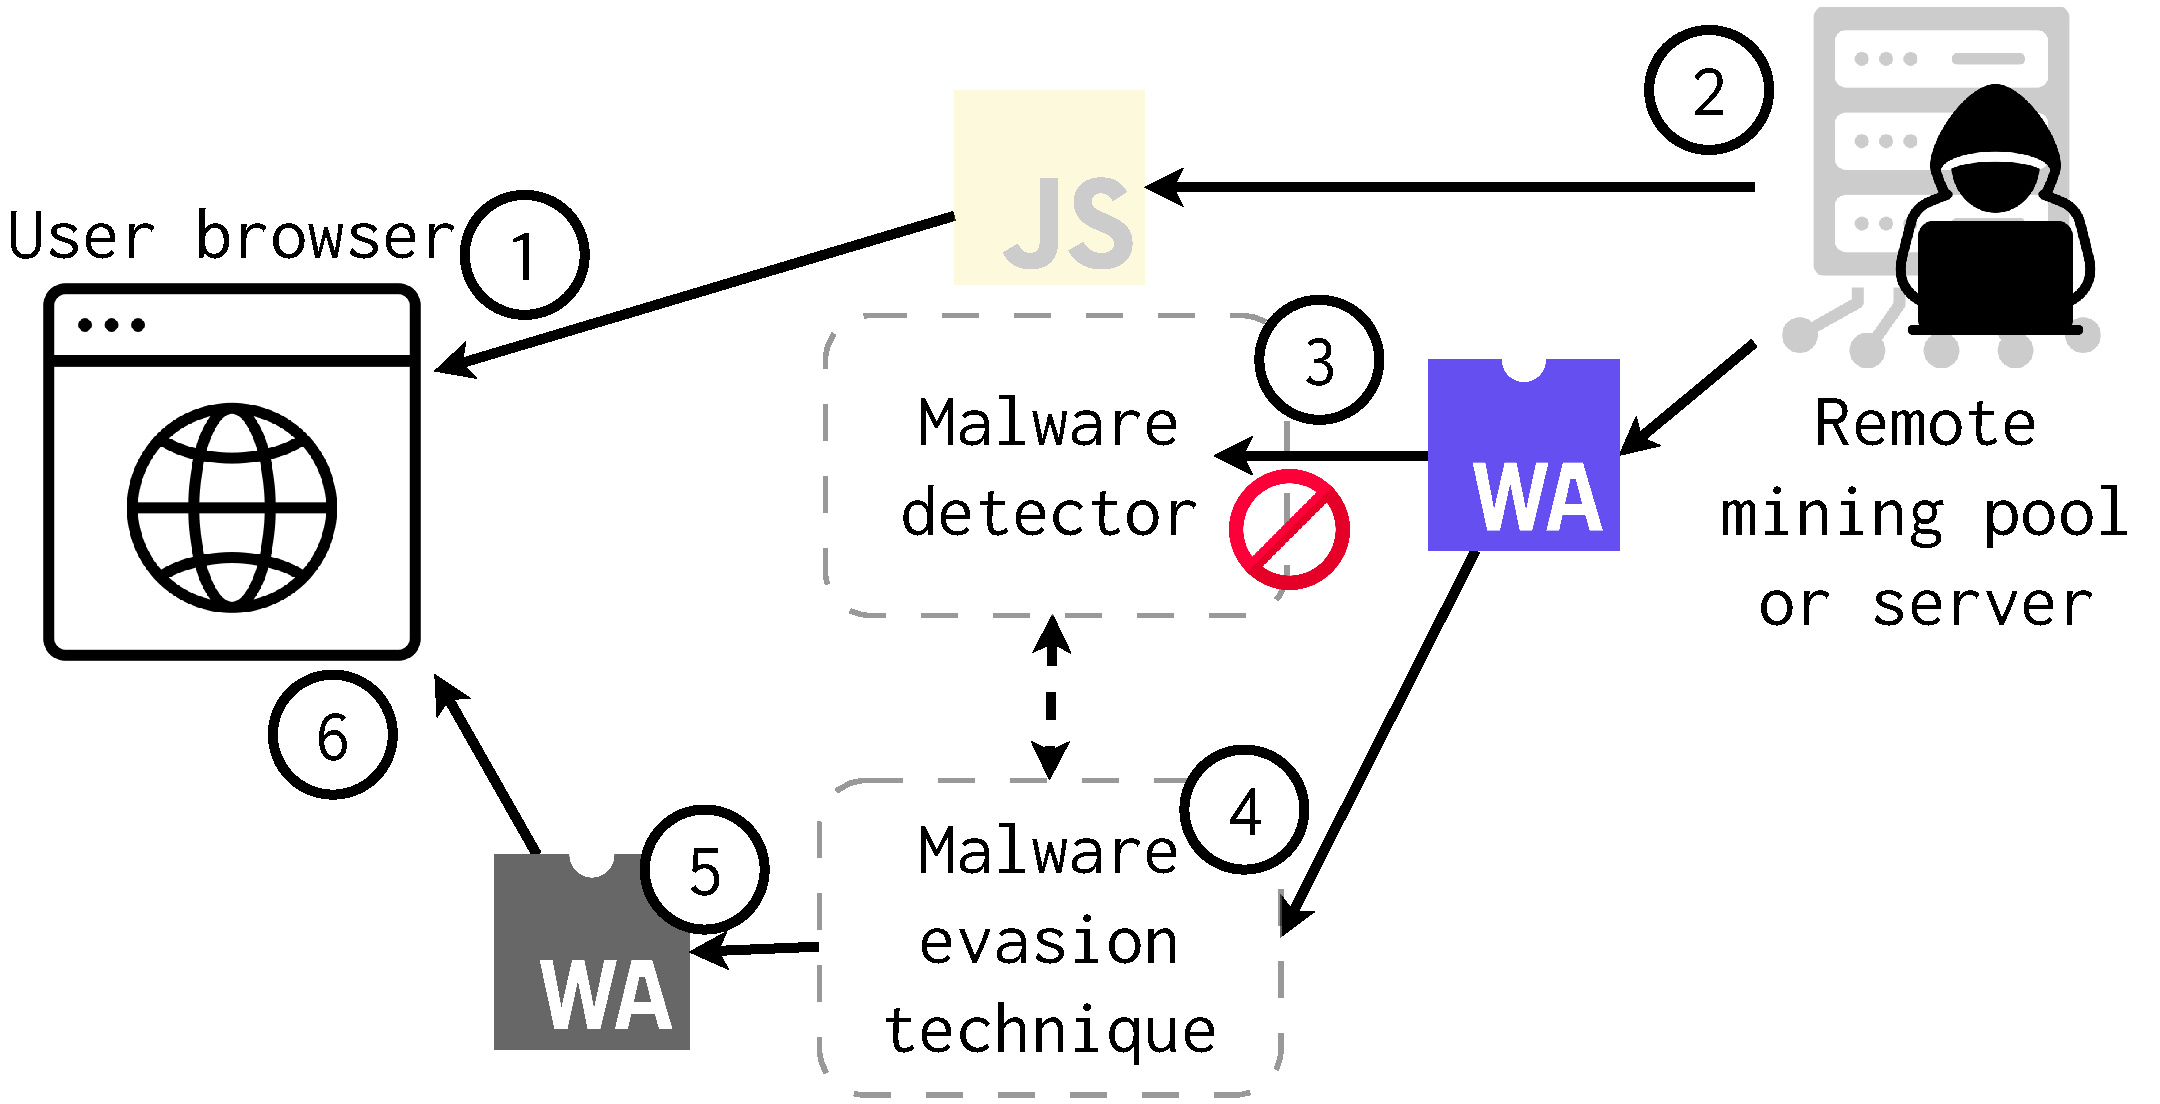
\includegraphics[width=0.8\linewidth]{figures/threat_model.pdf}
    \caption{Cryptojacking scenario in which the malware detection mechanism is bypassed by using an evasion technique.}
    \label{fig:threat_model}
\end{figure}


\begin{enumerate}
    
    \item The user loads a webpage infected with cryptojacking malware, which leverages network resources for execution—corresponding to \step{1} and \step{2} in \autoref{fig:threat_model}. 
    
    \item A malware detection mechanism (malware oracle) identifies and blocks malicious WebAssembly binaries at \step{3}. 
    For example, a network proxy could intercept and forward these resources to an external detection service via its API.
    
    \item Anticipating that a specific malware detection system is consistently used for defense, the attacker swiftly generates a variant of the WebAssembly cryptojacking malware designed to evade detection at \step{4}.
    
    \item The attacker delivers the modified binary instead of the original one \step{5}, which initiates the cryptojacking process and compromises the browser \step{6}. The detection method is not capable of detecting the malicious nature of the binary, and the attack is successful.
    
\end{enumerate}


\msubsection{Methodology}

Our aim is to validate, empirically, the effectiveness of Offensive Software Diversification in evading malware detection systems.
To achieve this, we employ WASM-MUTATE for generating \Wasm malware variants, with the goal of evading.
In this study, we categorize malware detection mechanisms as malware oracles, which can be of two types: binary and numeric. 
A binary oracle provides a binary decision, labeling a \Wasm binary as either malicious or benign. 
In contrast, a numeric oracle returns a numerical value representing the confidence level of the detection.

\begin{definition}{Malware oracle:}
    \label{malware_oracle_def}
    A malware oracle is a detection mechanism that returns either a binary decision or a numerical value indicating the confidence level of the detection.
\end{definition}


For empirical validation, we employ VirusTotal as a numeric oracle and MINOS \cite{MINOS} as a binary oracle. 
VirusTotal is an online service that analyzes files and returns a confidence score in the form of the number of antivirus that flag the input file as malware, thus qualifying as a numeric oracle. 
MINOS, on the other hand, converts \Wasm binaries into grayscale images and employs a convolutional neural network for classification. 
It returns a binary decision, making it a binary oracle.


We use the wasmbench dataset \cite{Hilbig2021AnES} to establish a ground truth. 
After running the wasmbench dataset through VirusTotal and MINOS, we identify 33 binaries that are: 1) flagged as malicious by at least one VirusTotal vendor and, 2) are also detected by MINOS.
Then, to simulate the evasion scenario, we use WASM-MUTATE to generate \Wasm binary variants to evade malware detection.
We use WASM-MUTATE in two configurations: controlled and stochastic diversification.

\begin{definition}{Feedback-guided Diversification:}
    \label{controlled_def}
    In feedback-guided diversification, the transformation process of a \Wasm program is guided by a numeric oracle, which influences the probability of each transformation. For instance, WASM-MUTATE can be configured to apply transformations that minimize the oracle's confidence score. Note that feedback-guided diversification needs a numeric oracle.
\end{definition}


\begin{definition}{Stochastic Diversification:}
    \label{uncontrolled_def}
    Unlike feedback-guided diversification, in stochastic diversification, each transformation has an equal likelihood of being applied to the input \Wasm binary.
\end{definition}


Based on the two types of malware oracles and diversification configurations, we examine three scenarios:
1) VirusTotal with a feedback-guided diversification, 2) VirusTotal with an stochastic diversification, and 3) MINOS with a stochastic diversification.
Notice that, the fourth scenario with MINOS and a feedback-guided diversification is not feasible, as MINOS is a binary oracle and cannot provide the numerical values required for feedback-guided diversification.

Our evaluation focuses on three key metrics: the success rate of evading detection mechanisms in VirusTotal and MINOS across the 33 flagged binaries, the correctness of the generated variants, and the performance impact on the variants that successfully evade detection.
The first metric measures the efficacy of WASM-MUTATE in bypassing malware detection systems. 
For each flagged binary, we input it into WASM-MUTATE, configured with the selected oracle and diversification strategy. 
We then iteratively apply transformations to the output from the preceding step. 
This iterative process is halted either when the binary is no longer flagged by the oracle or when a maximum of 1000 stacked transformations have been applied (see \autoref{stack_transform}).
This process is repeated with 10 random seeds per binary to simulate 10 different evasion experiments per binary.
The second metric is crucial for validating the real-world applicability of WASM-MUTATE in evading malware detection. 
Specifically, if the evasion process significantly degrades the performance of the resulting binary compared to its original version, it becomes less likely to be employed in practical scenarios, such as cryptojacking.
For this, we execute, end-to-end, the variants that fully evade VirusTotal when generated with WASM-MUTATE in controlled and stochastic diversification configurations.
We select variants for which we could completely reproduce the three components in \autoref{fig:attack_crypto}.

\msubsection{Results}

In \autoref{offensive:results:fast}, we present a comprehensive summary of the evasion experiments presented in \cite{EVASION}, focusing on two oracles: VirusTotal and MINOS\cite{MINOS}. 
The table is organized into two main categories to separate the results for each malware oracle. 
For VirusTotal, we further subdivide the results based on the two diversification configurations we employ: stochastic and feedback-guided diversification. 
In these subsections, the columns indicate the number of VirusTotal vendors that flag the original binary as malware (\#D), the maximum number of successfully evaded detectors (Max. \#evaded), and the average number of transformations required (Mean \#trans.) for each sample. 
We highlight in bold text the values for which the stochastic diversification or feedback-guided diversification setups best, the lower, the better.
The MINOS section solely includes a column that specifies the number of transformations needed for complete evasion. 
The table has 33 + 1 rows, each representing a unique \Wasm malware study subject. 
The final row offers the median number of transformations required for evasion across our evaluated setups and oracles. 

\newcolumntype{t}{>{\columncolor{Gray}}r}
\begin{table}
    \footnotesize
    \centering
    \begin{tabular}{c | r | r l | r l | t }
        \hline
        & \multicolumn{5}{|c|}{VirusTotal} & MINOS\cite{MINOS} \\
        \hline
        Hash & \#D & \multicolumn{2}{c|}{Stochastic diversification} & \multicolumn{2}{c|}{Feedback-guided diversification} & \\
        \hline
        &  & Max. #evaded & Mean #trans. & Max. #evaded & Mean #trans. & Mean #trans. \\
        \hline\hlined
        47d29959 &                 31 &             \textbf{26} &     N/A & 19 & N/A  & 100  \\ 
        9d30e7f0 &                 30 &             \textbf{24}  &      N/A & 17 & N/A & 419  \\ 
        8ebf4e44 &                 26 &             \textbf{21} &     N/A  & 13 & N/A & 92 \\
        \hline
        c11d82d &                 20 &       20        &  \textbf{355} & 20 & 446 & 115 \\ 
        0d996462 &                 19 &     19    &  \textbf{401} & 19 & 697 & 24 \\ 
        a32a6f4b &                 18 &       18       &  635 & 18 & \textbf{625} & 1 \\
        
        
        fbdd1efa &                 18 &         18      &  \textbf{310} & 18 & 726 & 1 \\ 
        d2141ff2 &                  9 &          9      &  \textbf{461} & 9 & 781 & 81 \\ 
        aafff587 &                  6 &          6      &  484 & 6 & \textbf{331} & 1 \\
        
        
        046dc081 &                  6 &          6      &  404 & 6 & \textbf{159} & 33 \\ 
        643116ff &                  6 &          6      &  \textbf{144} & 6 & 436 & 47 \\ 
        15b86a25 &                  4 &          4      &  253 & 4 & \textbf{131} & 1 \\
        
        
        
        006b2fb6 &                  4 &           4     &  \textbf{282} & 4 & 380 & 1\\ 
        942be4f7 &                  4 &           4     &  200 & 4 & 200 & 29\\ 
        7c36f462 &                  4 &           4     &  236 & 4 & \textbf{221} & 85\\
        
        
        fb15929f &                  4 &            4    &  \textbf{297} & 4 & 475 & 1 \\ 
        24aae13a &                  4 &         4       &  \textbf{252 } & 4 & 401 & 980\\ 
        000415b2 &                  3 &         3       &  302 & 3 & \textbf{34} & 960 \\
        
        4cbdbbb1 &                  3 &          3      &  295 & 3 & \textbf{72} & 1\\ 
        65debcbe &                  2 &          2      &  131  & 2 & \textbf{33} & 38 \\ 
        59955b4c &                  2 &          2      &  130  & 2 & \textbf{33} & 38 \\
        
        
        89a3645c &                  2 &           2     &  431 & 2 & \textbf{107} & 108\\
        a74a7cb8 &                  2 &           2     &  124 & 2 & \textbf{33} & 38 \\
        119c53eb &                  2 &           2     &  104 & 2 & \textbf{18} & 1 \\
        
        089dd312 &                  2 &           2     &  153 & 2 & \textbf{123} & 68\\
        c1be4071 &                  2 &           2     &  130 & 2 & \textbf{33} & 38\\
        dceaf65b &                  2 &           2     &  140 & 2 & 132 & 66\\
        
        6b8c7899 &                  2 &            2    &  143 & 2 & \textbf{33} & 38 \\
        a27b45ef &                  2 &         2       &  145 & 2 & \textbf{33} & 33\\
        68ca7c0e &                  2 &         2       &  137  & 2 & \textbf{33} & 38\\
        
        f0b24409 &                  2 &         2       &  127  & 2 & \textbf{11} & 33 \\
        5bc53343 &                  2 &         2       &  118  & 2 & \textbf{33} & 33 \\
        e09c32c5 &                  1 &         1       &  \textbf{120}  & 1 & 488 & 15 \\
        \hline\hline
        Median &                         &         &      218  &   & 131 & 38
    \end{tabular}
    \caption{
        The table has two main categories for each malware oracle, corresponding to the two oracles we use: VirusTotal and MINOS. 
        For VirusTotal, divide the results based on the two diversification configurations: stochastic and feedback-guided diversification. 
        We provide columns that indicate the number of VirusTotal vendors that flag the original binary as malware (\#D), the maximum number of successfully evaded detectors (Max. \#evaded), and the average number of transformations required (Mean \#trans.) for each sample. 
        We highlight in bold text the values for which diversification setups are best, the lower, the better.
        The MINOS section includes a column that specifies the number of transformations needed for complete evasion. 
        The final row offers the median number of transformations required for evasion across our evaluated setups and oracles. 
    }
    \label{offensive:results:fast}
\end{table}

\begin{strategy}[Stochastic diversification to evade VirusTotal]
    \label{stochastic_div_vt}
    We execute a stochastic diversification with WASM-MUTATE, setting a limit of 1000 iterations for each binary. 
    In every iteration, we query VirusTotal to determine if the newly generated binary can elude detection. 
    We repeat this procedure with ten distinct seeds for each binary, replicating ten different evasion experiments. 
    As the stochastic diversification section of \autoref{offensive:results:fast} illustrates, we successfully produce variants that fully evade detection for 30 out of 33 binaries. 
    The average amount of iterations required to produce a variant that evades all detectors oscillates between 120 to 635 stacked transformations. 
    The mean number of iterations needed never exceeds 1000 stacked transformations. 
    However, three binaries remain detectable under the stochastic diversification setup. 
    In these instances, the algorithm fails to evade 5 out of 31, 6 out of 30, and 5 out of 26 detectors. 
    This shortfall can be attributed to the maximum number of iterations, 1000, that we employ in our experiments. 
    Increasing iterations further, however, seems unrealistic. 
    If certain transformations enlarge the binary size, a significantly large binary could become impractical due to bandwidth limitations. 
    In summary, stochastic diversification with WASM-MUTATE markedly reduces the detection rate by VirusTotal antivirus vendors for cryptojacking malware, achieving total evasion in 30 out of 33 (90\%) cases within the malware dataset. 
    %WASM-MUTATE proves capable of successfully evading detection systems in just a few minutes.    
\end{strategy}
    

\begin{strategy}[Feedback-guided diversification to evade VirusTotal]
    \label{guided_div_vt}
    stochastic diversification does not guide the diversification based on the number of evaded detectors, it is purely random, and has some drawbacks.
    For example, some transformations might suppress other transformations previously applied.
    We have observed that, by carefully selecting the order and type of transformations applied, it is possible to evade detection systems in fewer iterations.
    This can be appreciated in the results of the feedback-guided diversification part of \autoref{offensive:results:fast}.
    The feedback-guided diversification setup successfully generates variants that totally evade the detection for 30 out of 33 binaries, it is thus as good as the stochastic setup.
    Remarkably, for 21 binaries out of 30, feedback-guided needs only 40\% of the calls the stochastic diversification setup needs, demonstrating larger efficiency. 

    %In practice, a potential attacker may be limited by budget on the number of transformations applicable to the malware binary, e.g., the number of queries to VirusTotal. 
    %Additionally, the performance of the resulting binary benefits from this approach.

\end{strategy}
  
\begin{strategy}[Stochastic diversification to evade MINOS]
    \label{stochastic_div_minos}
    Relying exclusively on VirusTotal for detection could pose issues, particularly given the existence of specialized solutions for \Wasm, which differ from the general-purpose vendors within VirusTotal. 
    In \autoref{background:wasm:analysis} we highlight several examples of such solutions.
    Yet, for its simplicity, we extend this experiment by using MINOS\cite{MINOS}, an antivirus specifically designed for \Wasm. 
    The results of evading MINOS can be seen in the final column of \autoref{offensive:results:fast}.
    The bottom row of \autoref{offensive:results:fast} highlights that fewer iterations are required to evade MINOS than VirusTotal through WebAssembly diversification, indicating a greater ease in eluding MINOS.
    The stochastic diversification setup requires a median iteration count of 218 to evade VirusTotal. 
    In contrast, the feedback-guided diversification setup necessitates only 131 iterations. 
    Remarkably, a mere 38 iterations are needed for MINOS. 
    In tests against MINOS, WASM-MUTATE evaded detection for 8 out of 33 binaries in a single iteration. 
    This result implies a vulnerability in the MINOS model to binary diversification.
\end{strategy}

\begin{strategy}[Meta-oracles]
    \label{meta-oracles}
    Our experiments indicate that VirusTotal surpasses MINOS in detecting \Wasm cryptojacking. 
    The primary factor contributing to this is VirusTotal's utilization of a broader range of antivirus vendors, which employs various detection strategies. 
    On the other hand, MINOS functions as a binary oracle. 
    This evidence supports the use of multiple malware oracles (meta-oracles) in identifying cryptojacking malware in browsers. 
    In the context of \Wasm, given the existence of numerous and diverse Wasm-specific detection mechanisms, this strategy is both practical and feasible, yet not explored in the literature.
\end{strategy}
    
%\msubsection{Efficiency and correctness results}

\begin{strategy}[\Wasm variants correctness]
    \label{evasion_impact}
    To evaluate the correctness of the malware variants created with WASM-MUTATE, we focused on six binaries that we could build and execute end-to-end, as these had all three components outlined in \autoref{fig:attack_crypto}. 
    We select only six binaries because the process of building and executing the binaries involves three components. 
    As detailed in \autoref{fig:attack_crypto}, they include the \Was binary, its JavaScript complement, and the miner pool. 
    These components were not found for the remaining 24 evaded binaries in the study subjects.
    For the six binaries, we then replace the original WebAssembly code with variants generated using VirusTotal as the malware oracle and WASM-MUTATE for both controlled and stochastic diversification configurations. 
    We then execute both the original and the generated variants. 
    We assess the correctness of the variants by examining the hashes they generate.
    If a minerpool detects a variant's generated hash as incorrect, or if the variant crashes during execution, we conclude an incorrect variant is created.
    Our findings show that all variants generated with WASM-MUTATE are correct, i.e., they generate the correct hashes and execute without error.
    Additionally, we found that 19\% of the generated variants surpassed the original cryptojacking binaries in performance.
\end{strategy}

\begin{tcolorbox}[title=Contribution paper,boxrule=1pt,arc=.2em,boxsep=1.0mm]
    WASM-MUTATE generates correct and performant variants of WebAssembly cryptojacking that successfully evade malware detection.
    The case discussed in this section is fully detailed in Cabrera-Arteaga \etal "WebAssembly Diversification for Malware Evasion"
    \emph{at Computers \& Security, 2023}
    \url{https://www.sciencedirect.com/science/article/pii/S0167404823002067}. 
\end{tcolorbox}


% Efficiency
%We have found that 
%This improvement is attributed to WASM-MUTATE's ability to introduce code optimizations. 
%Additionally, debloating transformations, which eliminate unnecessary structures and dead code, resulted in a higher hash generation rate during the initial seconds of mining, likely due to faster compilation times. 
%This suggests that focused optimization serves as a valuable tool for evasion in browsers.
% The contrary case.
%On the contrary, 80\% of the generated variants are less efficient than the original binary, with the least efficient variant operating at only 20\% of the original hash generation rate. 
%This performance drop is primarily due to non-optimal transformations introduced by WASM-MUTATE. 
%Variants generated through stochastic diversification are generally slower.
%In summary, feedback-guided diversification yielded variants that evaded VirusTotal detection with minimal performance overhead—the worst-performing variant was only 1.93 times slower than the original.


\msection{Defensive Diversification: Speculative Side-channel protection}

As previously discussed in \autoref{background:wasm:ecosystems}, \Wasm is rapidly gaining traction in backend environments. 
Companies like Cloudflare and Fastly are encouraging the use of \Wasm in their edge computing platforms, allowing developers to deploy faster applications in a modular and securely sandboxed fashion. 
Typically, these client \Wasm applications are designed as isolated services with a single, focused responsibility.
This model is usually called Function-as-a-Service (FaaS) \cite{pMendkiServerless, 1244493Jacobsson}.

The core concept behind \wasm in FaaS platforms is the ability to host thousands of client \Wasm binaries within a single host process, which is then distributed across multiple servers and data centers. 
To achieve this, the platforms compile the \wasm programs to native code, which is then executed in a sandboxed environment.
Then, the host processes are capable of instantiating a new Wasm sandbox for each client function, executing it in response to individual user requests in a matter of nanoseconds. 
Utilizing \Wasm enables these platforms to inherently isolate the execution of client functions from one another as well as from the host process.
However, this isolation is not foolproof against Spectre attacks \cite{Spectre,Narayan2021Swivel}.


In the subsequent sections, we illustrate how diversification can be used to protect \Wasm binaries against Spectre attacks.
We show a case of Defensive Software Diversification for the sake of protecting \Wasm binaries. 

\msubsection{Threat model: speculative side-channel attacks}

Let us illustrate the threat model in which a \Wasm program could be susceptible in FaaS platforms.
Developers can submit any \Wasm binary to the FaaS platform.
This includes potential malicious actors that could upload a \wasm binary that, when compiled to native code, uses Spectre attacks to leak sensitive information from the host process.
Spectre attacks exploit hardware predictors to induce misspredictions and speculatively execute instructions—gadgets that would not run sequentially. 
The attacker could then use this information to infer the contents of the memory of other client functions, or even the host process itself.

Narayan and colleagues \cite{Narayan2021Swivel} dissected the possible Spectre attacks for \wasm binaries into three categories based on the specific hardware predictor that is exploited and the specific FaaS scenario: Sandbox breakout attacks, Sandbox poisoning attacks and Host poisoning attacks.
The first one, exploits the branch target buffer by predicting the target of an indirect jump, thereby rerouting speculative control flow to an arbitrary target.
The second one takes advantage of the pattern history table to anticipate the direction of a conditional branch during the ongoing evaluation of a condition.
The third and last one exploits the return stack buffer that stores the locations of recently executed call instructions to predict the target of \texttt{ret} instructions. 
Each attack methodology relies on the extraction of memory bytes from another hosted \wasm binary that executes in the same host process.



\todo{Add diagram}
\todo{Explain here the threat model with the diagram}

%\lipsum[1]

%\lipsum[1]

\msubsection{Approach}
%\lipsum[1]

- Use of wasm-mutate

\msubsection{Results}

- Diminshing of BER
- Rockiki paper on portable side channel in browsers.



\todo{TBD discuss deoptimization}
% \subsection{Deoptimization}

\subsection{Partial input/output validation}

% We need to talk about this because, we do this checking right noe and it is probably a reason for the low count of variants.
When \tool generates a variant, it can be executed to check the input/output equivalence.
If the variant has a \_start function, both binaries, the original and the variant can be initialized. 
If the state of the memory, the globals and the stack is the same after executing the \_start function, they are partially equivalent.
%This mechanismm is already implemented in the fuzzing campaign of wasmtime.

The \_start function is easier to execute given its signature.
It does not receive parameters.
Therefore, it can be executed directly.
Yet, since a \Wasm program might contain more than one function that could be indistinctly called with and arbitrary number of parameters, we are not able to validate the whole program.
Thus, we call the checking of the initialization of a \wasm variant, a partial validation.

\subsection{Some other works to be cited along with the paper. Mostly in the Intro}

\emph{Spectre and side-channel defenses}

- paper 2021: Read this, since it is super related, \url{https://www.isecure-journal.com/article_136367_a3948a522c7c59c65b65fa87571fde7b.pdf} \cite{WasmSpectre}


- A dataset of Wasm programs: \cite{nicholson2023wasmizer}

- Papers 2020

- Papers 2019
- \cite{10.1145/3510003.3510070}

Selwasm: A code protection mechanism for webassembly


Babble

- https://arxiv.org/pdf/2212.04596.pdf

Principled Composition of Function Variants for Dynamic
Software Diversity and Program Protection

- https://dl.acm.org/doi/10.1145/3551349.3559553

How Far We’ve Come – A Characterization Study of Standalone WebAssembly Runtimes

- https://ieeexplore.ieee.org/document/9975423

Code obfuscation against symbolic execution attacks

Code artificiality: A metric for the code stealth based on an n-gram model

Semantics-aware obfuscation scheme prediction for binary

Wobfuscator: Obfuscating javascript malware via opportunistic translation to webassembly

Synthesizing Instruction Selection Rewrite Rules from RTL using SMT
"We also synthesize integer rewrite rules from WebAssembly to RISC-V "

Wafl: Binary-only webassembly fuzzing with fast snapshots



\begin{tcolorbox}[title=Contribution paper,boxrule=1pt,arc=.2em,boxsep=1.0mm]
    The case discussed in this section is fully detailed in Cabrera-Arteaga \etal "WASM-MUTATE: Fast and Effective Binary Diversification for WebAssembly"
    \emph{Under review}
    \url{https://arxiv.org/pdf/2309.07638.pdf}. 
\end{tcolorbox}




\msection{Intrinsic properties of diversification}
\label{exploit:discussion}
In \autoref{exploit:defensive}, we have noted an increasing trend of exfiltration bandwidth in certain variants. 
\autoref{offensive_app} presents a similar case, indicating that without a clear objective in the diversification process, uncontrolled diversification can be counterproductive. 
This implies that not all transformations contribute equally to the diversification objectives of \Wasm.
In the following, we elaborate on three cornerstones properties for improving Software Diversification with relation to \Wasm.

\wrule{Preservation:}
Some transformations yield distinct \Wasm binaries, yet their JIT compilation produces identical machine code.
Non-preserved transformations undermine the effectiveness of diversification, as discussed in \autoref{discussion}.
Incorporating random \texttt{nop} operations directly into \Wasm, for instance, does not alter the final machine code because JIT compilers typically eliminate these \texttt{nop} operations.
This phenomenon is also observed with transformations to the custom sections of \Wasm binaries.
Identical machine code, even when their \Wasm variants are different, can be detected by malware detectors.
For practitioners, malware detection tools can be enhanced by incorporating a pre-compilation step to normalize \Wasm binaries.
Besides, developers could focus on transformations that preserve the machine code, as they are more likely to contribute to the diversification objectives, e.g., evasion.
On the other hand, side-channel attacks occur at the machine code level.
Thus, making \Wasm variants preservation is essential code for successful defensive diversification, i.e., if the machine code is preserved, the side-channel attack will not be effective against the \Wasm variant.


%\wrule{Dead code addition:} 
%Transformed code may not always execute. 
%For example, Software Diversification might generate dead code or introduce a new function that the original program does not execute. 
%This is beneficial for static analysis, whether for avoiding reverse engineering or proving static malware detection. 
%However, dynamic analysis tools can identify this type of variant, e.g., this might reduce the effectiveness of evasion. 
%Furthermore, the inclusion of non-executing dead code does not affect side-channels.
%When the variant executes, it behaves identically to the original program, thereby not strengthening against potential attacks.
 
% More fine grained
\wrule{Disrupting timers:} Cache timing side-channel attacks, including for the four binaries analyzed in \autoref{exploit:defensive}, depend on precise timers to measure cache access times. 
Disrupting these timers can effectively neutralize the attack \cite{JStimers}. 
The \Wasm variants inherently adopt a similar approach, introducing perturbations in the timing steps of \Wasm variants. 
This is illustrated in \autoref{example:timer} and \autoref{example:timer2}, where the former shows the original time measurement and the latter presents a variant with introduced operations.
By introducing additional instructions, the inherent randomness in the time measurement of a single or a few instructions is amplified, thereby reducing the timer's accuracy. 


\lstdefinestyle{watcode}{
  numbers=none,
  stepnumber=1,
  numbersep=10pt,
  tabsize=4,
  showspaces=false,
  breaklines=true, 
  showstringspaces=false,
    moredelim=**[is][{\btHL[fill=weborange!40]}]{`}{`},
    moredelim=**[is][{\btHL[fill=celadon!40]}]{!}{!}
}


   \begin{minipage}[b]{\linewidth}
    \lstset{
        language=WAT,
                        style=watcode,
        basicstyle=\footnotesize\ttfamily,
                        columns=fullflexible,
                        breaklines=true}
        
        \begin{lstlisting}[label=example:timer,caption={Wasm timer code.},frame=b, captionpos=b]{Name}
;; Code from original btb_breakout
...
(call $readTimer)
(set_local $end_time)
... access to mem
(i64.sub (get_local $end_time ) (get_local $start_time))
(set_local $duration)
...

        \end{lstlisting}
\end{minipage}


\begin{minipage}[b]{\linewidth}
    \lstset{
        language=WAT,
                        style=watcode,
        basicstyle=\footnotesize\ttfamily,
                        columns=fullflexible,
                        breaklines=true}
        
        \begin{lstlisting}[label=example:timer2,caption={\Wasm variant with more instructions added in between time measurement.},frame=b, captionpos=b]{Name}
;; Variant code
...
(call $readTimer)
(set_local $end_time)
!<inserted instructions>!
... access to mem
!<inserted instructions>!
(i64.sub (get_local $end_time ) (get_local $start_time))
(set_local $duration)
...
        \end{lstlisting}
\end{minipage}


\todo{Recheck term-citation padding here}

\wrule{Padding speculated instructions:} CPUs have a limit on the number of instructions they can cache. 
Diversification injects instructions to potentially exceed this limit, effectively disabling the speculative execution of memory accesses. 
This approach is akin to padding \cite{padding}, as demonstrated in \autoref{example:padding} and \autoref{example:padding2}.
This padding disrupts the binary code's layout in memory, hindering the attacker's ability to initiate speculative execution. 
Even if speculative execution occurs, the memory access does not proceed as the attacker intended.


\lstdefinestyle{watcode}{
  numbers=none,
  stepnumber=1,
  numbersep=10pt,
  tabsize=4,
  showspaces=false,
  breaklines=true, 
  showstringspaces=false,
    moredelim=**[is][{\btHL[fill=weborange!40]}]{`}{`},
    moredelim=**[is][{\btHL[fill=celadon!40]}]{!}{!}
}


   \begin{minipage}[b]{0.8\linewidth}
    \lstset{
        language=WAT,
                        style=watcode,
        basicstyle=\footnotesize\ttfamily,
                        columns=fullflexible,
                        breaklines=true}
        
        \begin{lstlisting}[label=example:padding,caption={Two jump locations. The top one trains the branch predictor, the bottom one is the expected jump that exfiltrates the memory access.},frame=b, captionpos=b]{Name}
;; Code from original btb_breakout
...
;; train the code to jump here (index 1)
(i32.load (i32.const 2000))
(i32.store (i32.const 83)) ;; just prevent optimization
...
;; transiently jump here
(i32.load (i32.const 339968)) ;; S(83) is the secret
(i32.store (i32.const 83)) ;; just prevent optimization
        \end{lstlisting}
\end{minipage}


\begin{minipage}[b]{0.8\linewidth}
    \lstset{
        language=WAT,
                        style=watcode,
        basicstyle=\footnotesize\ttfamily,
                        columns=fullflexible,
                        breaklines=true}
        
        \begin{lstlisting}[label=example:padding2,caption={\Wasm variant with more instructions added indindinctly between jump places.},frame=b, captionpos=b]{Name}
;; Variant code
...
;; train the code to jump here (index 1)
!<inserted instructions>!
(i32.load (i32.const 2000))
!<inserted instructions>!
(i32.store (i32.const 83)) ;; just prevent optimization
...
;; transiently jump here
!<inserted instructions>!
(i32.load (i32.const 339968)) ;; "S"(83) is the secret
!<inserted instructions>!
(i32.store (i32.const 83)) ;; just prevent optimization
...
        \end{lstlisting}
\end{minipage}






% \msection{Threats to validity}
\label{threats}

We discuss the threats to the validity of the two use cases presented in this chapter.
We separate the threats to validity into three main categories: internal, external, and construct validity.

\msubsection{Internal validity}


\msubsection{External validity}


\msubsection{Construct validity}


\subsection{Partial input/output validation}

% We need to talk about this because, we do this checking right noe and it is probably a reason for the low count of variants.
When \tool generates a variant, it can be executed to check the input/output equivalence.
If the variant has a \_start function, both binaries, the original and the variant can be initialized. 
If the state of the memory, the globals and the stack is the same after executing the \_start function, they are partially equivalent.
%This mechanismm is already implemented in the fuzzing campaign of wasmtime.

The \_start function is easier to execute given its signature.
It does not receive parameters.
Therefore, it can be executed directly.
Yet, since a \Wasm program might contain more than one function that could be indistinctly called with and arbitrary number of parameters, we are not able to validate the whole program.
Thus, we call the checking of the initialization of a \wasm variant, a partial validation.


\section*{Conclusions}

In this chapter, we discuss two sides of Software Diversification as applied to \Wasm: Offensive Software Diversification and Defensive Software Diversification.
Offensive Software Diversification underscores both the capabilities and the latent security risks inherent in applying Software Diversification to \Wasm malware.
Our research indicates that there are ways for enhancing the automated detection of cryptojacking malware in WebAssembly, e.g. by stressing their resilience with \Wasm malware variants.
On the other hand, Defensive Software Diversification acts as a preemptive safeguard, specifically to mitigate the risks posed by Spectre attacks.
In the subsequent chapter, we will consolidate the principal conclusions of this dissertation and describe directions for future research.